\subsection{Style extraction and handwriting reproduction}
\label{sec:des-reproduction}
Recognition returns text, but the gantry needs pen paths. The reproduction stage extracts reusable glyphs from labelled handwriting, stores each writer's shape and spacing measurements, and assembles them into new text.

\subsubsection{Choice of reproduction representation}
A glyph profile reuses the few labelled pages available for each writer. Haines et al. used approximately four A4 pages in their standard glyph-based experiments~\cite[p.~4]{haines2016}. The explicit paths can be inspected, resized and mapped to the gantry without training another generator.

The photographs contain no measured pen order, speed or pressure, unlike the trajectories required by recurrent synthesis~\cite[p.~18]{graves2013}. Image generators can use few style references, but still need a separate training corpus. One-DM's IAM experiment used 339 writers and four RTX 3090 GPUs~\cite[p.~9]{dai2024}. The chosen glyph approach fits the available data and compute, with weaker handling of letter shapes that change with their neighbours.

\subsubsection{Character alignment and glyph extraction}
\label{sec:des-alignment}
A source line has a known transcript but no character-position labels. The reader supplies frame probabilities, and forced alignment selects the highest-scoring path consistent with that transcript. It uses the CTC transition rules, replacing path summation with maximisation~\cite[pp.~4--5]{graves2006}.
\begin{equation}
V(t,s)=\log p_t(\ell'_s)+\max_{r\in\mathcal P(s)}V(t-1,r).
\label{eq:des-viterbi}
\end{equation}

Here $\ell'$ is the blank-interleaved transcript and $\mathcal P(s)$ is the permitted predecessor set for state $s$. Backtracking gives each character's frame interval. A frame edge $t$ maps approximately to source position $(640t/T)/a$, using the inverse canvas scale $a$. Several plausible boundaries can still give the correct transcript.

The horizontal ink profile estimates the body band. Its first and last rows above 45\% of the maximum define the band top and baseline $b$, with difference $h_x$ giving estimated x-height. Bands below three pixels are rejected. Initial character cuts are refined towards thin connectors or blank columns using the project-specific cost
\begin{equation}
C_x=\frac{\overline p_x}{q_{0.60}(\{\overline p_j:\overline p_j>0\})}
+1.15\operatorname{clip}\left(\frac{b-y_{\mathrm{top}}(x)}{h_x},0,3\right).
\label{eq:des-cutcost}
\end{equation}

where $\overline p_x$ is smoothed column ink, the denominator is its positive-count 60th percentile, and $y_{\rm top}(x)$ is the highest ink row. The height term favours shallow connectors near the baseline. A true blank column has zero cost. Cuts remain ordered, with minimum cell width $\max(1,0.08h_x)$, so neighbouring boundaries cannot collapse onto the same gap.

Figure~\ref{fig:des-alignment} follows the archived first Owen line because its crop and transcript can be traced through recognition and extraction. It shows the initial frame locations, refined cuts and resulting glyphs. The worked path and cut-cost substitutions are in Appendix~\ref{app:worked-design-calculations}.
\begin{figure}[H]\centering
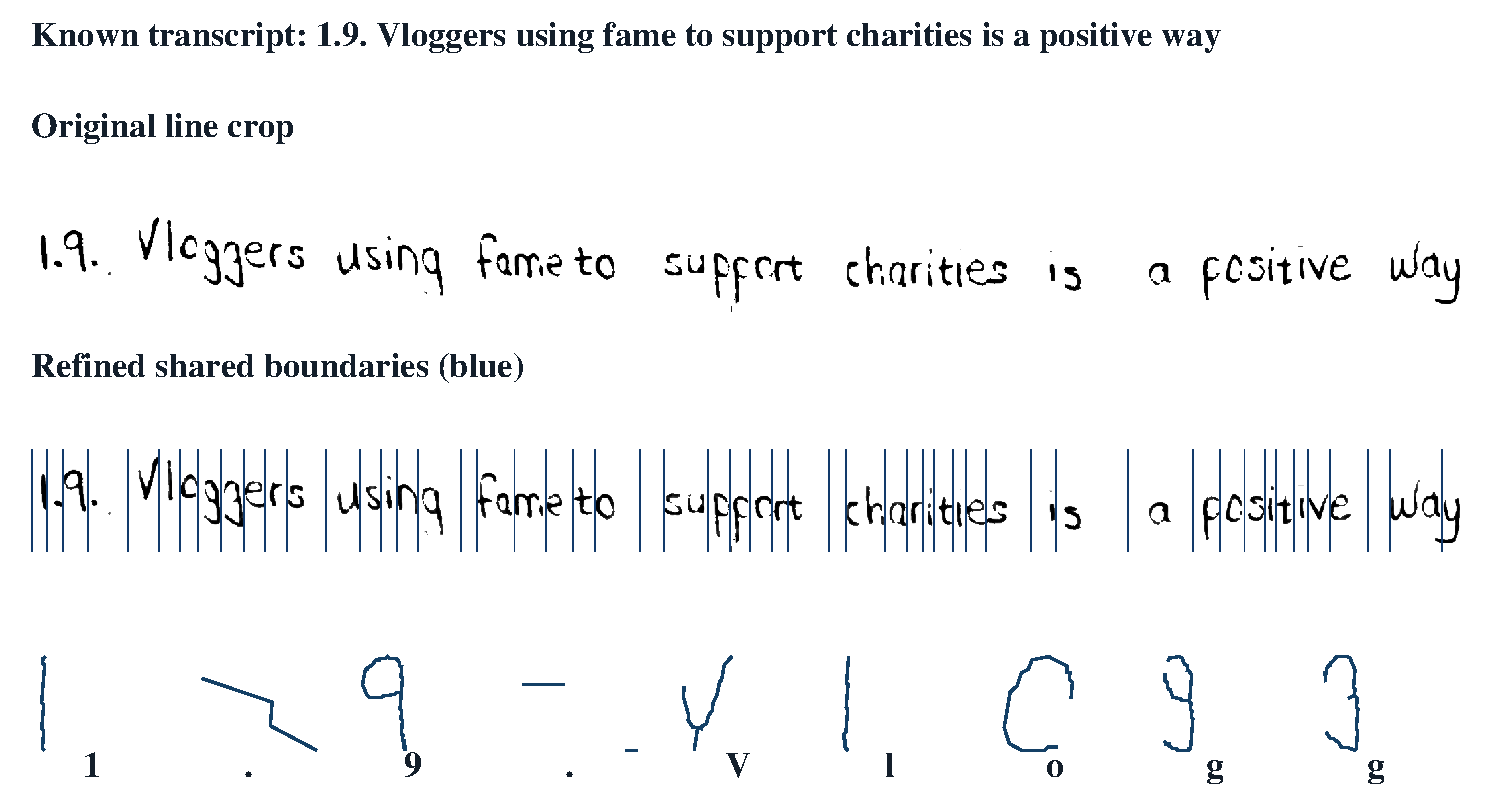
\includegraphics[width=\linewidth]{Figures/design-glyph-alignment.pdf}
\caption{Character alignment and refined glyph cuts.}
\label{fig:des-alignment}
\end{figure}

\subsubsection{Skeleton tracing and pen path construction}
Thinning converts ink area into a one-pixel centreline~\cite[p.~237]{zhang1984}. The complete line is thinned before cutting it into cells, avoiding an artificial thinning boundary at every letter. A graph tracer splits paths at junctions, prunes short spurs and rejoins compatible ends below a $75^\circ$ continuation angle. Douglas--Peucker simplification removes unnecessary vertices within a bounded deviation~\cite{douglas1973}.

Isolated dots are recovered as short paths. Eligible detached crossbars are assigned to their letter rather than split across cells or counted as cursive joins. The resulting points are stored relative to left cut $x_L$, baseline $b$, x-height $h_x$ and slant $\phi$, using a shear transform~\cite{vinciarelli2001}.
\begin{equation}
v=\frac{b-y}{h_x},\qquad
u_0=\frac{x-x_L}{h_x}-v\tan\phi,\qquad u=u_0-\delta.
\label{eq:des-glyphcoords}
\end{equation}

The vertical coordinate increases upwards. The trim shift $\delta$ is removed from the stored horizontal path and retained as lead-in spacing. Slant is removed for storage and reapplied at placement. This separates the letter shape from its source size and cell spacing.

Figure~\ref{fig:vt-tracing} shows the Owen fragment before and after thinning and tracing. Across its full line, simplification reduces 3738 vertices to 974 at 0.6 source-pixel tolerance. The graph gives geometric paths, while the writer's original stroke order remains unknown. The coordinate substitution is retained in Appendix~\ref{app:worked-design-calculations}.
\begin{figure}[H]\centering
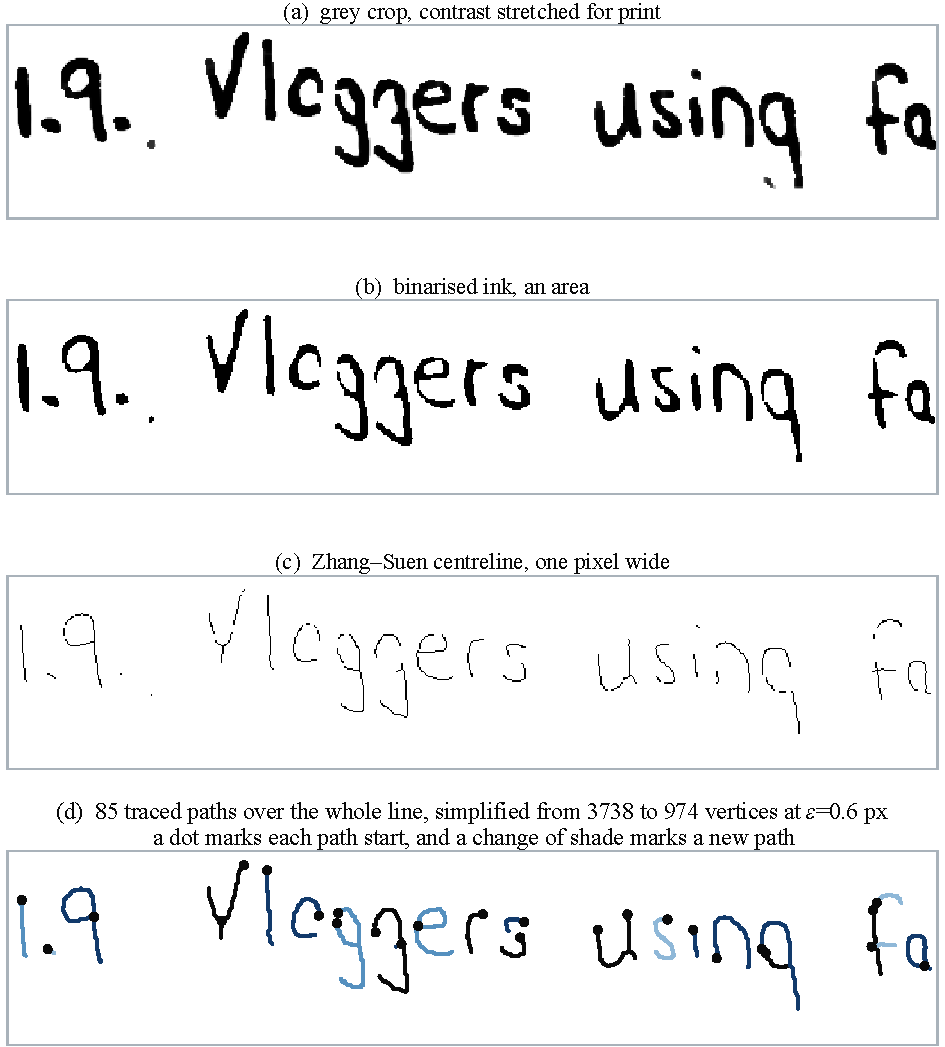
\includegraphics[width=\linewidth]{Figures/VisualTests/T41_skeleton_trace_simplify.pdf}
\caption{Ink, skeleton and simplified pen paths.}
\label{fig:vt-tracing}
\end{figure}

\subsubsection{Glyph selection and library quality}
Alignment can place a cut inside a letter even when the text is correct. The profile therefore filters unreliable lines and glyphs using width, height, stroke count, path length and allocated character advance. Ordinary widths are limited to 2.1 x-heights and wide letters to 2.9. Character-specific distributions provide further checks without forcing every letter to the same size.

A normalised $12\times12$ occupancy descriptor compares shape. A pooled character reference identifies malformed cuts, while pairwise distances within a writer's pool identify a representative real variant, called the medoid. A separate denoised prototype combines compatible strokes. The ordinary pool holds up to twelve variants per character. Algorithm~\ref{alg:des-profile} shows where these checks enter profile construction. The descriptor distance is $d(g,c)=1-v_g^Tr_c$ for unit-normalised glyph descriptor $v_g$ and class reference $r_c$. The medoid minimises summed within-class distances.
\begin{designalgorithm}
\caption{Labelled handwriting to a persistent writer profile}
\label{alg:des-profile}
\prequire{Labelled original lines $\mathcal L$, trained reader and writer identifier.}
\begin{designpseudo}
\pstate{0}{$\mathcal G\leftarrow\varnothing$; $\mathcal S\leftarrow\varnothing$}
\pstate{0}{\textbf{for each} $(G,\ell)\in\mathcal L$ \textbf{do}}
\pstate{1}{$A\leftarrow\operatorname{ForcedAlign}(G,\ell)$; estimate baseline, x-height and slant}
\pstate{1}{\textbf{if} alignment or body band is unusable \textbf{then continue}}
\pstate{1}{Refine shared increasing cuts; thin full line; trace skeleton paths}
\pstate{1}{Split paths at cuts; assign crossbars; recover untraced dots}
\pstate{1}{Normalise glyph coordinates; record advance, lead and boundary crossings}
\pstate{1}{Append glyphs to $\mathcal G$ and line measurements to $\mathcal S$}
\pstate{0}{\textbf{end for}}
\pstate{0}{Cache raw extraction; reject low-confidence lines relative to this writer}
\pstate{0}{\textbf{for each} character's glyph pool $\mathcal G_c$ \textbf{do}}
\pstate{1}{Apply size, height-class, path-length and cell-consistency gates}
\pstate{1}{Refine size range; apply cross-writer prior and within-writer consensus}
\pstate{1}{Rank and smooth retained variants; construct medoid and eligible prototype}
\pstate{0}{\textbf{end for}}
\pstate{0}{\textbf{return} persistent profile containing $\mathcal G$ and robust summaries of $\mathcal S$}
\end{designpseudo}
\end{designalgorithm}

Figure~\ref{fig:des-profile-example} compares the nine stored \texttt{a} variants for Owen, Dylan and Yeukita. The cloud shows their variation, the medoid is an actual example, and the prototype is a combined shape. The distance bars explain which variant is most typical within each writer. The exact descriptor and medoid calculations are retained in Appendix~\ref{app:worked-design-calculations}.
\begin{figure}[H]\centering
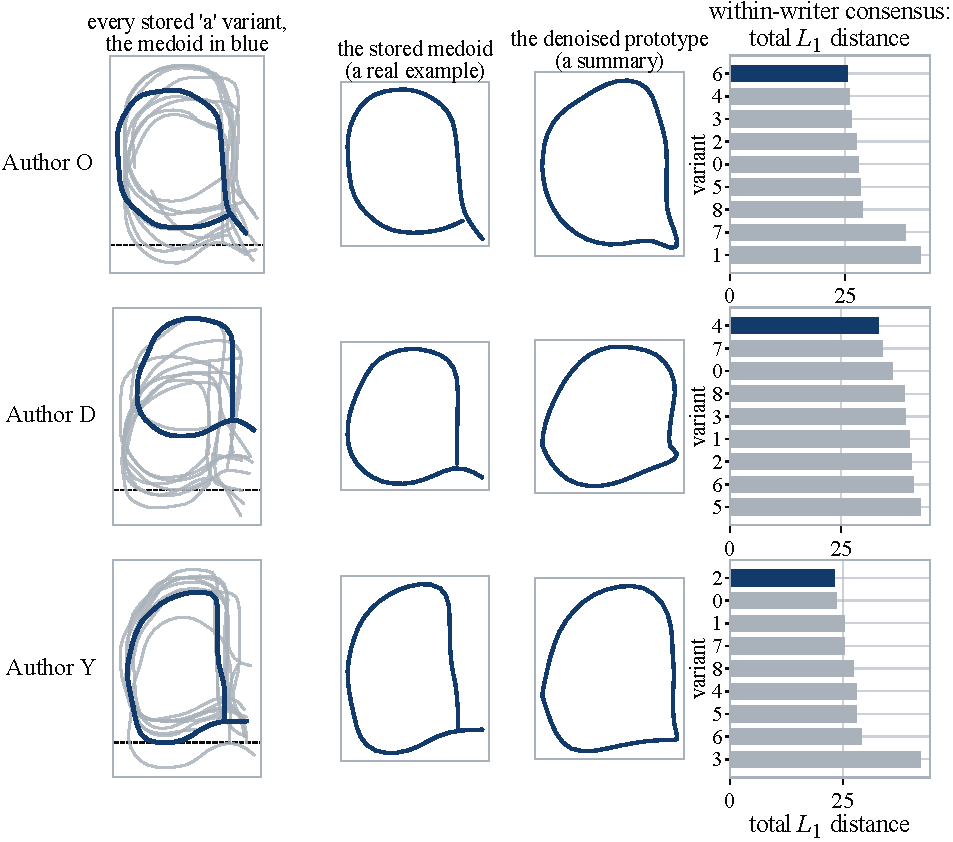
\includegraphics[width=\linewidth]{Figures/VisualTests/T45_variant_pool_medoid.pdf}
\caption{Glyph variants and representatives for three writers.}
\label{fig:des-profile-example}
\end{figure}

Missing characters can use case-related shapes, similar forms or fallback glyphs. Source tags distinguish these choices from observed personal letterforms. They allow text generation to continue, but a fallback does not establish that the character was captured in that writer's style.

\subsubsection{Writer style measurement and storage}
\label{sec:des-profile}
The profile stores slant, x-height, ascender and descender extent, character advance, word gap and connection fraction. Slant is estimated by finding the shear that concentrates ink into columns. Dimensions are normalised by x-height to reduce dependence on photograph resolution.

Connectedness is the fraction of eligible adjacent non-space boundaries crossed by a traced centreline, motivated by contour-based writer features~\cite[p.~701]{bulacu2007}.
\begin{equation}
c=\frac{N_{\mathrm{cross}}}{\max(1,N_{\mathrm{adj}})}.
\label{eq:des-connectedness}
\end{equation}

The Owen example has 3 crossings among 39 eligible boundaries, giving 0.077. This is a property of the source ink, not a measured pen-lift sequence. Glyph paths and style measurements are stored together under the writer identity for later requests.

\subsubsection{Text layout and connected handwriting synthesis}
\label{sec:des-layout}
The synthesiser selects glyph variants, applies the stored style and places words within the available line width. Character advance and word gap come from the profile. Words wrap to the next line when the remaining width is insufficient.

For stored point $(u,v)$ and lead $l$, physical x-height $h_x^{\rm mm}$ converts the glyph to millimetres. Slant shear $s$ and baseline drift $d$ are applied about placement origin $(p_x,p_y)$.
\begin{equation}
x=p_x+h_x^{\mathrm{mm}}(l+u+sv),\qquad
y=p_y+h_x^{\mathrm{mm}}(v+d).
\label{eq:des-placement}
\end{equation}

Small translations, rotations and scale changes provide variation. Drift changes gradually with persistence 0.85 and is bounded to $\pm0.25$ x-heights. A nominal 0.05 x-height clearance limits collisions. Better-ranked variants are sampled more often, with compatible entry heights preferred for joining.

The automatic anchoring strength $\lambda$ depends on median stored prior distance $\widetilde d$.
\begin{equation}
\lambda=\operatorname{clip}\left(\frac{\widetilde d-0.24}{0.32-0.24},0,1\right).
\label{eq:des-anchor}
\end{equation}

Lower-distance pools retain more personal variants. Larger distances increase reliance on an acceptable representative and then a generic form if needed. This is a heuristic, with source tags recording the resulting glyph choice.

Joining uses the writer's measured connection fraction, but is suppressed below 0.45. A join also requires a compatible source and gap no greater than 0.80 x-heights. A shallow connector joins the body strokes without attaching to dots or crossbars. A rendered probe applies bounded slant and extent corrections before synthesis. The placement and anchoring examples are retained in Appendix~\ref{app:worked-design-calculations}.

\subsubsection{Candidate selection for legibility and writer identity}
\label{sec:des-selection}
Different variant choices can change readability and writer identity. Each candidate is rendered at constant ink width and scored by the reader and stroke-normalised writer classifier. Character score $A$ and requested-writer probability $P$ form joint score $J$.
\begin{equation}
A=\max\left(0,1-\frac{d_{\mathrm{edit}}(\widehat t,t)}{|t|}\right),\qquad
J=\begin{cases}2AP/(A+P),&A+P>0,\\0,&\text{otherwise}.\end{cases}
\label{eq:des-jointscore}
\end{equation}

The harmonic mean penalises a candidate weak in either score. The recorded Owen candidate has $A=18/19=0.95$ and $P=0.58$, giving $J=0.72$. Algorithm~\ref{alg:des-joint} gives the bounded search and repair sequence. A repair is retained only when the complete candidate score improves.
\begin{designalgorithm}
\caption{Joint candidate search and bounded legibility repair}
\label{alg:des-joint}
\prequire{Text, writer profile, reader, shape classifier, seed $s$ and trial budget $K$.}
\begin{designpseudo}
\pstate{0}{$J^*\leftarrow-1$; $R\leftarrow\varnothing$; determine anchoring strength}
\pstate{0}{\textbf{for} $k\leftarrow0$ \textbf{to} $\max(1,K)-1$ \textbf{do}}
\pstate{1}{$T\leftarrow\operatorname{SynthesizeText}(\text{text},\text{profile},s+977k)$}
\pstate{1}{$I\leftarrow\operatorname{RenderUniformInk}(T)$; $(A,P,J)\leftarrow\operatorname{Score}(I)$}
\pstate{1}{\textbf{if} $J>J^*$ \textbf{then} $(T^*,I^*,J^*)\leftarrow(T,I,J)$}
\pstate{1}{\textbf{if} $J^*\geq0.99$ \textbf{then break}}
\pstate{0}{\textbf{end for}}
\pstate{0}{\textbf{for} at most three configured repair rounds \textbf{do}}
\pstate{1}{\textbf{if} $J^*\geq0.995$ \textbf{then break}}
\pstate{1}{$W\leftarrow$ up to two weak aligned positions not already in $R$}
\pstate{1}{\textbf{if} $W=\varnothing$ \textbf{then break}}
\pstate{1}{$R'\leftarrow R\cup W$; regenerate with stronger anchors at $R'$ and seed $s$}
\pstate{1}{Render and rescore the complete trial trajectory}
\pstate{1}{\textbf{if} $J>J^*$ \textbf{then} commit $R'$ and the new best trajectory}
\pstate{0}{\textbf{end for}}
\pstate{0}{\textbf{return} $T^*$ with selection and accepted-repair metadata}
\end{designpseudo}
\end{designalgorithm}

Figure~\ref{fig:des-candidates} compares the three recorded trials of ``Writing with style.'' using the same profile and settings. Candidate 1 is selected because its writer score is stronger while retaining the same character score as candidate 3. The full values are in Appendix~\ref{app:worked-design-calculations}.
\begin{figure}[H]\centering
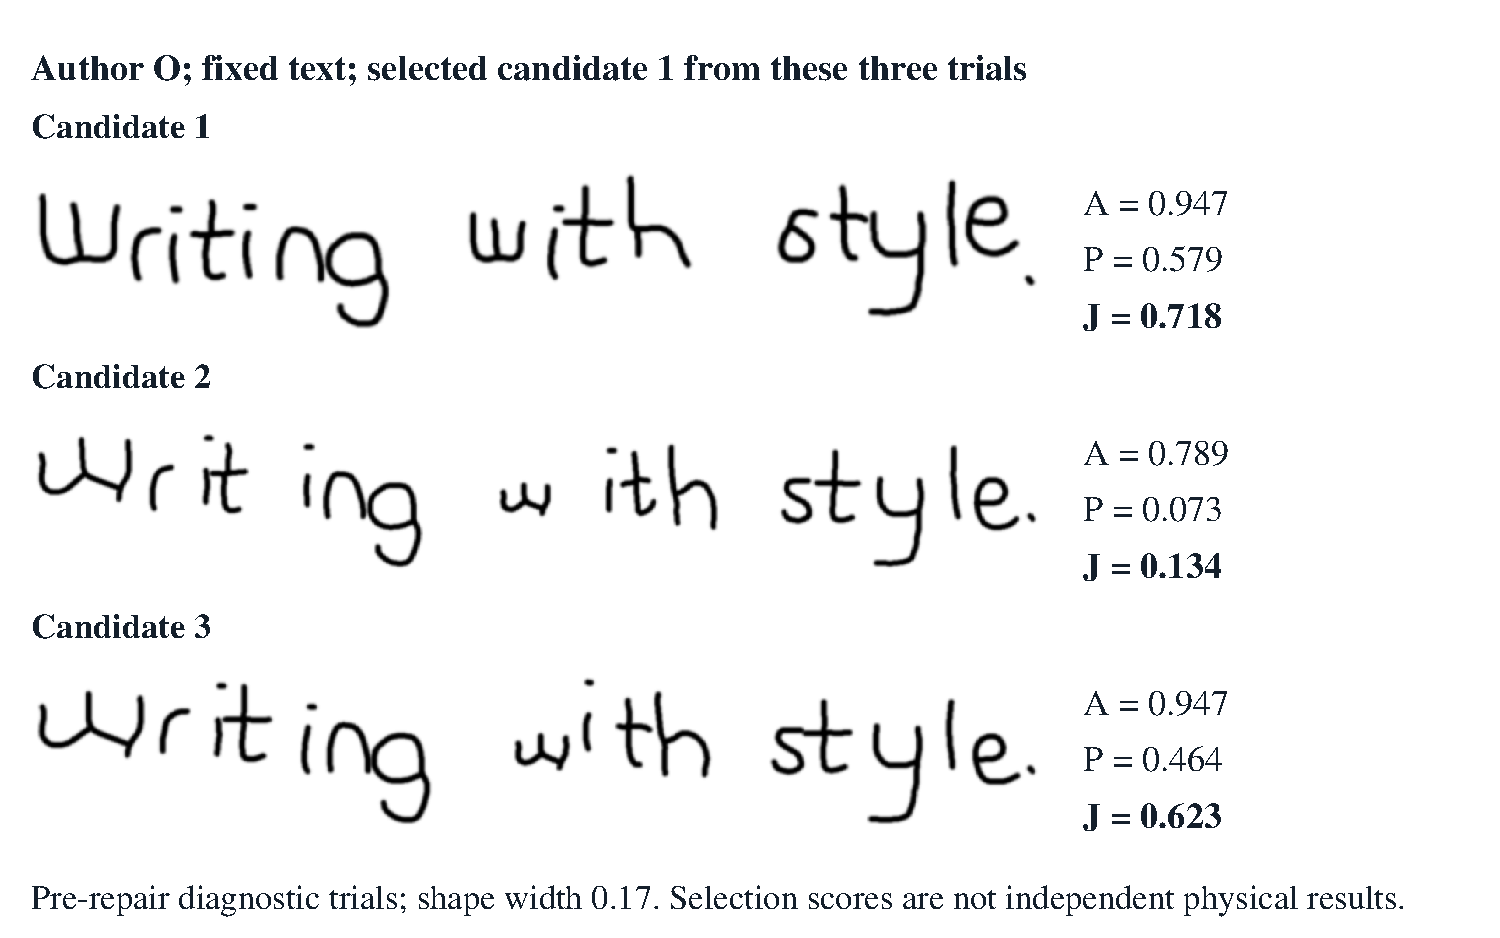
\includegraphics[width=\linewidth]{Figures/design-candidate-selection.pdf}
\caption{Candidate paths and their selection scores.}
\label{fig:des-candidates}
\end{figure}

The scoring models guide this choice, so their confidence does not independently prove physical style similarity. More trials also add inference time and cannot recover a missing source letterform.

\subsubsection{Machine coordinate mapping and G-code generation}
\label{sec:des-gcode}
The selected trajectory is fitted inside the calibrated workspace. Ruled placement adjusts each line to the chosen ruling, while free placement retains its synthesised pitch. Character size and line spacing remain separate so that a tall descender need not change both.

Trajectory bounds $(x_0,y_0,x_1,y_1)$, origin $(o_x,o_y)$, margins $m_x,m_y$ and scale $a$ define the mapping. Offset $d_y$ selects a later starting line and $\Delta_y$ adjusts line spacing.
\begin{equation}
x_m=o_x+m_x+a(x-x_0),\qquad
y_m=o_y-m_y-d_y-a(y_1-y)+\Delta_y.
\label{eq:des-machinecoords}
\end{equation}

Both stored and machine coordinates use upward-increasing $y$. Clamping is a final travel limit and can distort a letter. Robust extent fitting and margins should keep the generated text inside the bed before execution. Nearby path segments may be simplified and compatible strokes joined, using a default join distance of 0.6\,mm.

Figure~\ref{fig:des-gcode-excerpt} gives the opening commands of the generated Owen example. It selects millimetres, absolute coordinates, a raised-pen travel and the first drawing movements. The full point mapping and file interpretation are extended in Appendix~\ref{app:worked-design-calculations}.
\begin{figure}[H]
\begin{lstlisting}[style=designcode]
G21
G90
G0 F2400
G0 F2400 X15.000 Y240.557
M3
G4 P0.350
G1 F900
G1 X15.001 Y240.207
G1 X15.002 Y239.857
G1 X15.003 Y239.506
G1 X15.005 Y239.156
G1 X15.006 Y238.806
G1 X15.007 Y238.456
\end{lstlisting}
\caption{Opening commands of the Owen example.}
\label{fig:des-gcode-excerpt}
\end{figure}

Travel feed is restated after drawing because feed is modal. Pen dwell adds 0.35\,s per transition to the switch-confirmed actuation. For drawing and travel distances $D_d,D_u$, feeds $F_d,F_u$ and $N_p$ alternating pen transitions, the nominal budget is
\begin{equation}
t_{\mathrm{nom}}=\frac{60D_d}{F_d}+\frac{60D_u}{F_u}
+\frac{N_p(t_{\mathrm{up}}+t_{\mathrm{down}})}{2}.
\label{eq:des-timebudget}
\end{equation}

The earlier traced file gives 32.82\,s, including 19.60\,s dwell. Figure~\ref{fig:vt-timeparts} shows a separate four-profile calculation for the same sentence. Dwell contributes about 61 to 65\% of these nominal budgets. This identifies a motion-side improvement to test, while actual completion also includes synthesis, actuation and pulse-loop overhead.
\begin{figure}[H]\centering
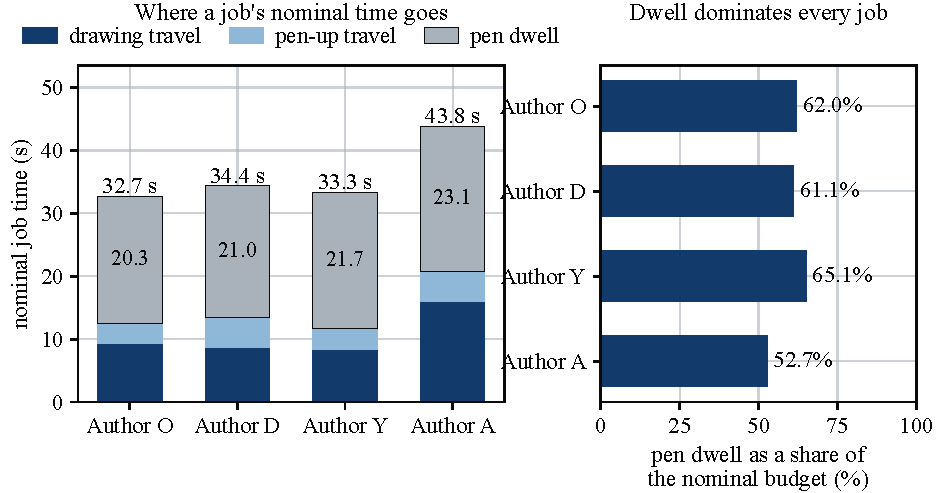
\includegraphics[width=\linewidth]{Figures/VisualTests/T56_time_budget.pdf}
\caption{Drawing, travel and pen-dwell budgets.}
\label{fig:vt-timeparts}
\end{figure}

\subsubsection{Reproduction verification and design limitations}
Checks follow source ink, stored glyphs, assembled paths and emitted G-code. The independent file parser in Appendix~\ref{app:des-visual-tests} recovers the generated paths. Nine controlled fixtures preserve vertex counts with maximum coordinate discrepancy 0.0004\,mm, consistent with three-decimal coordinate emission. Physical drawing tests then check the mechanism rather than file conversion alone.

The explicit glyph representation makes source errors and scaling inspectable. Its main limits are context-dependent letterforms, missing characters and the absence of natural pen dynamics. Multi-character units and recorded trajectories could address these losses, but need additional reliable data. Physical qualification remains in Results.
\FloatBarrier
